\graphicspath{{figures/analysis/}}
\chapter{Analysis}\label{ch:analysis}
An object tracking solutions consists of multiple steps towards creating complete trajectories for each object in an arena. As stated in \autoref{ch:related}, occlusions often lead to issues in tracking solutions and are often not handled to completion. This leads to missing data which a user must handle either by annotating some of the data themselves or using the data incomplete.

To combat this, some solutions choose to solve the occlusions \citep{Romero-Ferrero2019, Dolado2015}. By being able to detect when an occlusion occurs a process of handling them is initiated.

Both \cite{Romero-Ferrero2019} and \cite{Dolado2015} initially counts the amount of objects in the each frame and compare it to the given amount of object which are supposed to be in the frame.\\

An implementation of an occlusion detection solution can be categorised as a single step in an object tracking system. The detection step would consist of detecting occlusions in every frame, categorising the type of occlusion and extracting the occlusion position in the image. This is also show in an flowchart overview in \autoref{fig:overview_flow}.
%Problem analyse. Hvad er det jeg/vi vil løse og hvorfor? Skal lægge op til problem formuleringen.

Often, before any kind of detections take place some pre processing of the image is done \citep{Delcourt2018}. This would be any kind of alternations made to the image, which will make it easier to isolate the desired objects from the rest of the image.

An implementation of an occlusion detection solution must be placed before the tracking of the objects in a object tracking pipeline, as the handling of occlusions should be done before extracting positions of each individual in the image. An occlusion detection element of an object detection solution which should be able to distinguish between a single fish \gls{blob} and a \gls{blob} consisting of multiple fish.

If the occlusions are handled before doing any kind of tracking, the tracking solution will face less issues needing a solution to be able to track all objects.

\begin{figure}[H]
	\centering
	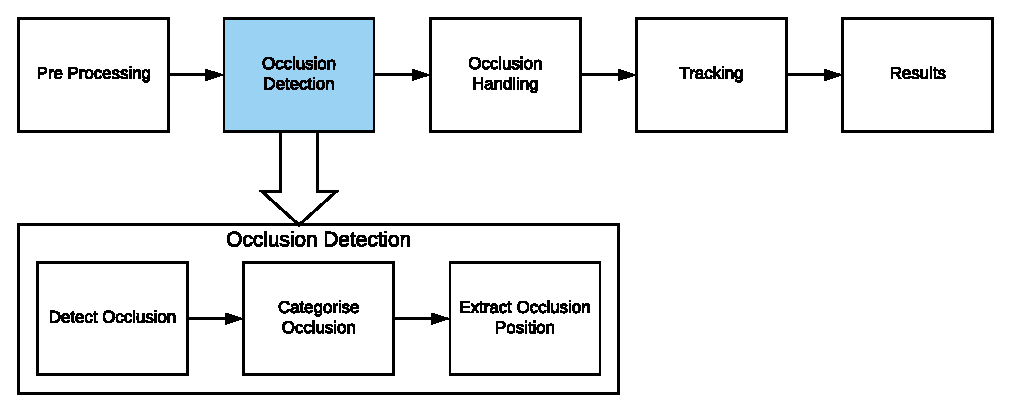
\includegraphics[width=\textwidth]{overview_flowchart}
	\caption{Overview of an entire tracking system solution and specification of the occlusion detection part.}
	\label{fig:overview_flow}
\end{figure}

An occlusion detection solution needs to be able to detect when and where an occlusion is occurring to be able to pass the information on to the occlusion handling process.
